\documentclass[10pt,twocolumn,letterpaper]{article}

\usepackage{iccv}
\usepackage{times}
\usepackage{epsfig}
\usepackage{graphicx}
\usepackage{calc}
\usepackage{amsmath}
\usepackage{amssymb}
\usepackage{tabu}
\usepackage{adjustbox}
\usepackage[percent]{overpic}
\usepackage[utf8]{inputenc}
\usepackage{pgfplots}
\DeclareUnicodeCharacter{2212}{−}
\usepgfplotslibrary{groupplots,dateplot}
\usetikzlibrary{patterns,shapes.arrows}
\pgfplotsset{compat=newest}

\usetikzlibrary{decorations.pathreplacing,calc,automata, shapes.geometric,shapes.arrows,decorations.pathmorphing,matrix,chains,scopes,positioning,arrows,fit}

\newcommand{\tikzmark}[2][-3pt]{\tikz[remember picture, overlay, baseline=-0.5ex]\node[#1](#2){};}


\usepackage[pagebackref=true,breaklinks=true,letterpaper=true,colorlinks,bookmarks=false]{hyperref}


\def\iccvPaperID{3600} %
\def\httilde{\mbox{\tt\raisebox{-.5ex}{\symbol{126}}}}

\ificcvfinal\pagestyle{empty}\fi

\definecolor{purple}{rgb}{1, 0, 1}

\newcommand{\ie}{\emph{i.e.,}\xspace}
\newcommand{\eg}{\emph{e.g.,}\xspace}
\newcommand{\abr}{\emph{abbr.}\xspace}
\newcommand{\ea}{\emph{et al.}\xspace}
\newcommand{\gensync}{\emph{GenSync}\xspace}
\newcommand{\colosseum}{\emph{Colosseum}\xspace}
\newcommand{\srep}{\emph{SREP}\xspace} % Set Reconciliation Enhances
\newcommand{\srepsim}{\emph{SREPSim}\xspace}
% Propagation
\newcommand{\esrep}{\emph{E-SREP}\xspace}
\newcommand{\epsrep}{\emph{EP-SREP}\xspace}
\newcommand{\mesrep}{\emph{ME-SREP}\xspace}
\newcommand{\mempoolsync}{\emph{MempoolSync}}

\newcommand{\fref}[1]{Fig.~\ref{#1}}
\newcommand{\tref}[1]{Table~\ref{#1}}
\newcommand{\aref}[1]{Algorithm~\ref{#1}}
\newcommand{\procref}[1]{Procedure~\ref{#1}}
\newcommand{\sref}[1]{Section~\ref{#1}}
\newcommand{\lineref}[1]{line~\ref{#1}}
\newcommand{\appref}[1]{Appendix~\ref{#1}}

% Change \eqref
\LetLtxMacro{\originaleqref}{\eqref}
\renewcommand{\eqref}{Eq.~\originaleqref}

% Theorems and corollaries
\newcounter{theoremcount}
\setcounter{theoremcount}{0}
\DeclareRobustCommand{\theorem}[1]{%
  \refstepcounter{theoremcount}%
  \noindent\textit{\textbf{Theorem \thetheoremcount\label{theorem:#1}: }}%
}
\DeclareRobustCommand{\theoremref}[1]{Theorem~\ref{theorem:#1}}

\DeclareRobustCommand{\proof}{\emph{Proof:}\xspace}
\DeclareRobustCommand{\qqed}{\hfill$\blacksquare$}

\newcounter{corollcount}
\setcounter{corollcount}{0}
\DeclareRobustCommand{\coroll}[1]{%
  \refstepcounter{corollcount}%
  \noindent\textit{\textbf{Corollary \thecorollcount\label{coroll:#1}: }}%
}
\DeclareRobustCommand{\corollref}[1]{Corollary~\ref{coroll:#1}}

\newcounter{lemmacount}
\setcounter{lemmacount}{0}
\DeclareRobustCommand{\lemma}[1]{%
  \refstepcounter{lemmacount}%
  \noindent\textit{\textbf{Lemma \thelemmacount\label{lemma:#1}: }}%
}
\DeclareRobustCommand{\lemmaref}[1]{Lemma~\ref{lemma:#1}}

\newcounter{definitioncount}
\setcounter{definitioncount}{0}
\DeclareRobustCommand{\definition}[1]{%
  \refstepcounter{definitioncount}%
  \noindent\textit{\textbf{Definition \thedefinitioncount\label{definition:#1}: }}%
}
\DeclareRobustCommand{\defref}[1]{Definition~\ref{definition:#1}}

%notes of different authors
\newif\ifnotes
\notestrue
\notesfalse

\newif\ifdiff
\difftrue
\difffalse

\newcommand{\anote}[1]{\ifnotes $\ll$\textsf{\textcolor{purple}{Ari: {#1}}}$\gg$ \fi}
\newcommand{\nnote}[1]{\ifnotes $\ll$\textsf{\textcolor{orange}{Novak: {#1}}}$\gg$ \fi}
\newcommand{\diff}[1]{\ifdiff\textcolor{orange}{#1}\else#1\fi}

%%% Local Variables:
%%% mode: latex
%%% TeX-master: "main"
%%% End:


\begin{document}

\title{Point2Vec for Self-Supervised Representation Learning on Point Clouds \\  Supplementary Material}


\author{First Author\\
Institution1\\
Institution1 address\\
{\tt\small firstauthor@i1.org}
\and
Second Author\\
Institution2\\
First line of institution2 address\\
{\tt\small secondauthor@i2.org}
}

\ificcvfinal\thispagestyle{empty}\fi
\maketitle

\begin{abstract}
This supplementary material contains further ablation studies on the efficiency of pre-training data and the selection of hyperparameters during pre-training and fine-tuning on downstream tasks.
Our code and model will be made publicly available for research purposes.
\end{abstract}

\section{Further Ablation Studies}

\paragraph{Pretext Task.}
In the main paper, we have only explored self-supervised pre-training on the ShapeNet dataset.
However, ShapeNet also contains class labels which could instead be used for a fully supervised classification-based pre-training.
As can be seen in \reftab{pretext_tasks}, this yields a significantly worse performance than using \name{} or even than directly training \emph{from scratch}.
We can also pre-train using \name{} directly on ModelNet40, which constitutes roughly a quarter of ShapeNet's size.
Still, we see improved downstream performances, indicating that the \name{} pretext task is meaningful for pre-training.

\paragraph{Warm-Up EMA Rate.}
During pre-training, we linearly warm-up the EMA rate $\tau$ over the first $\tau_n$ epochs from its initial value $\tau_0$ to its final value $\tau_e$ \,\cite{baevski2022data2vec}.
This approach is based on the idea that we should update the teacher network more frequently at the start of training since the feature representations are not yet well-established.
In\,\reftab{ema_tau_ablation}, we show overall accuracy scores on ModelNet40 and the \texttt{PB-T50-RS} variant of ScanObjectNN using various values for $\tau_n$.
Our findings suggest that $\tau_n$ is a crucial hyperparameter for achieving effective pre-training with \name{}.
In\,\reftab{hyperparameters}, we provide the EMA rates employed by our baseline \datavec{} and \name{}, respectively.
\begin{table}
    \centering
    \setlength{\tabcolsep}{2pt}
    \caption{
        \textbf{Pretext Tasks.}
        After pre-training with a classification objective on ShapeNet, fine-tuning on ModelNet40 leads to no performance gains over directly training \emph{from scratch} and significantly worse performance on the most difficult test split of ScanObjectNN.
        However, \name{} already brings performance gains when pre-trained with the much smaller ModelNet40 dataset and significant improvements when pre-trained with the large ShapeNet dataset.        
    }
    \label{tab:pretext_tasks}
    \begin{tabular}{lccc}
    	\toprule
    	         & \multicolumn{3}{c}{Overall Accuracy}                                \\
    	\cmidrule(lr){2-4}
    	         & \multicolumn{2}{c}{\textbf{ModelNet40}} & \textbf{ScanObjNN}        \\
    	\cmidrule(lr){2-3} \cmidrule(lr){4-4}
    	Pretext Task & $+$Voting                               & $-$Voting          &   \small \texttt{PB-T50-RS}   \\
    	\midrule
            none / from scratch & $93.3$ & $93.0$ & $84.3$ \\
            classification (ShapeNet) & $93.2$                                    & $93.0$ & $82.9$ \\
            \arrayrulecolor{black!10}\midrule\arrayrulecolor{black}
            \name{} (ModelNet40) & $93.9$ & $93.6$ & $84.4$ \\
    	\name{} (ShapeNet) & $\mathbf{94.8}$ & $\mathbf{94.7}$ & $\mathbf{87.5}$ \\
            \bottomrule
    \end{tabular}
\end{table}

\begin{table}
    \centering
    \caption{
        \textbf{Warm-Up EMA Rate.}
        We linearly warm-up the EMA rate during the first $\tau_n$ epochs.
    }
    \label{tab:ema_tau_ablation}
    \begin{tabular}{ccccc}
    	\toprule
    	         & \multicolumn{3}{c}{Overall Accuracy}                                \\
    	\cmidrule(lr){2-4}
    	         & \multicolumn{2}{c}{\textbf{ModelNet40}} & \textbf{ScanObjNN}        \\
    	\cmidrule(lr){2-3} \cmidrule(lr){4-4}
    	$\tau_n$ & $+$Voting                               & $-$Voting          &  \small \texttt{PB-T50-RS}    \\
    	\midrule
    	80       & 94.5                                    & 94.1               & 86.7 \\
            160      & 94.6                                    & 94.2               & 87.4 \\
            200      & \textbf{94.8}                           & \textbf{94.7}      & \textbf{87.5} \\
            300      & 94.1                                    & 94.0               & 87.3 \\
            400      & 94.0                                    & 94.0               & 87.3 \\
            \bottomrule
    \end{tabular}
\end{table}

\begin{figure*}
    \centering
    \subcaptionbox{Row-normalized confusion matrix}{
    \includegraphics[trim=0 0 30 0,width=0.48\textwidth]{figures/confusion_matrix/confusion_matrix_norm_true.pdf}
    }
    \subcaptionbox{Column-normalized confusion matrix}{
    \includegraphics[trim=0 0 30 0,width=0.48\textwidth]{figures/confusion_matrix/confusion_matrix_norm_pred.pdf}
    }
    \caption{
        \textbf{Confusion matrix of \name{} on the ModelNet40 test split.}
        We present the confusion matrix, both row-normalized (a) and column-normalized (b).
        The diagonals of these show the recall and precision respectively.
        As expected, the matrix reveals that the majority of misclassifications occur between a small number of closely related classes.
        The most frequent cases of misclassifications are `\emph{night\_stand}'s that are classified as `\emph{dresser}'s, `\emph{flower\_pot}'s that are classified as `\emph{plant}'s and `\emph{table}'s that are classified as `\emph{desk}'s.
    }
    \label{fig:modelnet_confusion}
\end{figure*}
\paragraph{Target Layer Aggregation.}
During training of \datavec{}, as well as \name{}, we need to specify which layers of the teacher should be defined as the target.
The target is constructed by averaging the last $K$ layers, where Baevski \etal \cite{baevski2022data2vec} recommend to use half the number of total layers in absence of additional experiments.
We ablate this hyperparameter and report results in \reftab{number_of_target_layers}.
Although all tested values lead to usable results, indeed $K=6$ overall leads to the best performance.
\begin{table}
    \centering
    \caption{
        \textbf{Target Layer Aggregation.}
        We construct training targets by averaging the outputs of the last $K$ Transformer blocks of the teacher.
        We observe that $K=6$ is optimal for ModelNet40 and close to optimal for the \texttt{PB-T50-RS} variant of ScanObjectNN.
    }
    \label{tab:number_of_target_layers}
    \begin{tabular}{ccccc}
    	\toprule
    	         & \multicolumn{3}{c}{Overall Accuracy}                                \\
    	\cmidrule(lr){2-4}
    	         & \multicolumn{2}{c}{\textbf{ModelNet40}} & \textbf{ScanObjNN}        \\
    	\cmidrule(lr){2-3} \cmidrule(lr){4-4}
    	$K$ & $+$Voting              & $-$Voting          &     \small \texttt{PB-T50-RS}   \\
    	\midrule
    	1      & 94.4                                    & 94.1               & 87.0 \\
            3      & 94.7                                    & 94.3               & 87.1 \\
            6      & \textbf{94.8}                           & \textbf{94.7}      & 87.5 \\
            9      & 94.3                                    & 94.0               & \textbf{87.6} \\
            12     & 94.5                                    & 94.3               & 87.3 \\
            \bottomrule
    \end{tabular}
\end{table}


\vspace{10pt}
\paragraph{Pre-Training Data Efficiency.}
\begin{figure}[t!]

\definecolor{darkorange25512714}{RGB}{255,127,14}
\definecolor{darkslategray38}{RGB}{38,38,38}
\definecolor{lightgray204}{RGB}{204,204,204}
\definecolor{steelblue31119180}{RGB}{31,119,180}

\begin{center}
\footnotesize
\begin{tabular}{cc}
{\color{darkorange25512714}\large \textbf{---}} Point-MAE\,\cite{pang2022pointmae} & {\color{steelblue31119180}\large \textbf{---}}  \textbf{\name{}} (Ours)
 \\
\hspace{2cm}&\hspace{2cm}
\end{tabular}
\end{center}
\vspace{-25px}
\hspace{-17px}

\subcaptionbox{ModelNet40\,\cite{wu2015modelnet40}}{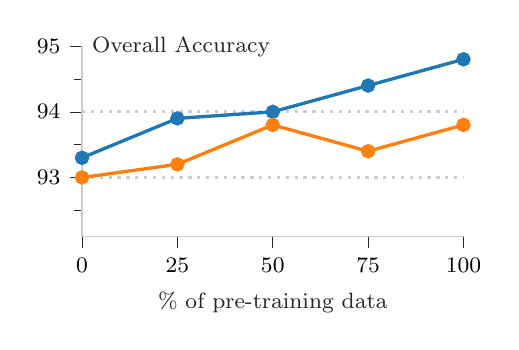
\begin{tikzpicture}

\definecolor{darkorange25512714}{RGB}{255,127,14}
\definecolor{darkslategray38}{RGB}{38,38,38}
\definecolor{lightgray204}{RGB}{204,204,204}
\definecolor{steelblue31119180}{RGB}{31,119,180}

\begin{axis}[
width=0.53\linewidth,height=4cm,
axis x line=bottom,
axis y line=left,
x axis line style={-},
ytick distance=0.5,
minor y tick num=1,
ytick={92, 93, 94, 95},
y axis line style={-},
axis line style={white!80!black},
legend cell align={left},
legend style={
  fill opacity=0.8,
  draw opacity=1,
  text opacity=1,
  at={(0.97,0.03)},
  anchor=south east,
  draw=lightgray204,
  legend image post style={line width =1.0pt}
},
tick align=outside,
xlabel=\textcolor{darkslategray38}{\footnotesize \% of pre-training data},
xmin=0, xmax=100,
xtick={0, 25, 50, 75, 100},
xtick style={color=darkslategray38},
y grid style={lightgray204},
x grid style={lightgray204},
every axis y label/.style={at={(0.001,1.1)},anchor=north west},
ylabel=\textcolor{darkslategray38}{\footnotesize Overall Accuracy},
ymin=92.1, ymax=95.0,
ytick style={color=darkslategray38},
tick label style={font=\footnotesize},
]

\addplot [very thick, dotted, lightgray204]
table {%
0 93
100 93
};

\addplot [very thick, dotted, lightgray204]
table {%
0 94
100 94
};

\addplot [very thick, steelblue31119180, mark=*, mark size=2, mark options={solid}]
table {%
0 93.3
25 93.9
50 94.0
75 94.4
100 94.8
};
\addplot [very thick, darkorange25512714, mark=*, mark size=2, mark options={solid}]
table {%
0 93.0
25 93.2
50 93.8
75 93.4
100 93.8
};

\end{axis}

\end{tikzpicture}}%
\hfill
\subcaptionbox{ScanObjectNN\,\cite{uy2019scanobjectnn}}{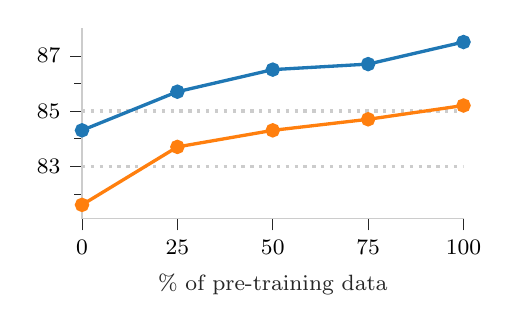
\begin{tikzpicture}

\definecolor{darkorange25512714}{RGB}{255,127,14}
\definecolor{darkslategray38}{RGB}{38,38,38}
\definecolor{lightgray204}{RGB}{204,204,204}
\definecolor{steelblue31119180}{RGB}{31,119,180}

\begin{axis}[
width=0.53\linewidth,height=4cm,
axis x line=bottom,
axis y line=left,
x axis line style={-},
ytick distance=0.5,
minor y tick num=1,
ytick={81, 83, 85, 87},
y axis line style={-},
axis line style={white!80!black},
legend cell align={left},
legend style={
  fill opacity=0.8,
  draw opacity=1,
  text opacity=1,
  at={(0.97,0.03)},
  anchor=south east,
  draw=lightgray204,
  legend image post style={line width =1.0pt}
},
tick align=outside,
xlabel=\textcolor{darkslategray38}{\footnotesize \% of pre-training data},
xmin=0, xmax=100,
xtick={0, 25, 50, 75, 100},
xtick style={color=darkslategray38},
y grid style={lightgray204},
x grid style={lightgray204},
every axis y label/.style={at={(0.001,1.0)},anchor=north west},
ymin=81.1, ymax=88.0,
ytick style={color=darkslategray38},
tick label style={font=\footnotesize},
]

\addplot [very thick, dotted, lightgray204]
table {%
0 83
100 83
};

\addplot [very thick, dotted, lightgray204]
table {%
0 85
100 85
};

\addplot [very thick, steelblue31119180, mark=*, mark size=2, mark options={solid}]
table {%
0 84.3
25 85.7
50 86.5
75 86.7
100 87.5
};
\addplot [very thick, darkorange25512714, mark=*, mark size=2, mark options={solid}]
table {%
0 81.6
25 83.7
50 84.3
75 84.7
100 85.2
};

\end{axis}

\end{tikzpicture}}%

\caption{
\textbf{Pre-training Data Efficiency.}
Irrespective of the quantity of pre-training data used from ShapeNet, \name{} consistently achieves better results than Point-MAE\,\cite{pang2022pointmae} on ModelNet40 (with voting) and the most difficult test split of ScanObjNN.
}
\label{fig:pretraining_data_efficiency}
\vspace{-20pt}
\end{figure}
We evaluate the efficiency of self-supervised pre-training with \name{}.
To this end, we partition the ShapeNet training dataset into subsets containing $25\%$, $50\%$, $75\%$ and $100\%$ of the data.
We then fine-tuned our model for shape classification on ModelNet40 and ScanObjectNN, respectively.
As shown in\,\reffig{pretraining_data_efficiency}, \name{} achieves consistent improvements on both datasets.
Notably, pre-training \name{} with only $25\%$ of the training data yields superior results compared to Point-MAE pre-trained with $100\%$ of the training data.

\paragraph{Class Confusions on ModelNet40.}
Given the very high overall accuracies on the ModelNet40 dataset, we further analyze the remaining errors.
\reffig{modelnet_confusion} shows the confusion matrix on the ModelNet40 test split, clearly showing that most remaining mistakes are made for a few classes with very similar appearances, which might also be difficult for humans to distinguish.


\section{Architecture Details.}


In \reftab{hyperparameters}, we provide detailed hyperparameters for pre-training \datavec{} and \name{} on ShapeNet.
We, furthermore, report the hyperparameters for fine-tuning \name{} for the shape classification (\reftab{hyperparameters_classification}) and part segmentation task (\reftab{hyperparameters_part_segmentation}).
In Listing \ref{lst:point2vec}, we provide the PyTorch-inspired pseudocode for \name{} pre-training.

\section{Qualitative Results for Part Segmentation.}
\begin{figure*}[t!]
\includegraphics[width=1.0\linewidth,trim={0cm 0.85cm 0cm 0.85cm},clip]{figures/shapenetpart_qualitative/part_qual.pdf}
\caption{
\textbf{Qualitative Results on ShapeNetPart.}
\name{} produces well localized boundaries between parts with minimal semantic errors.
In most cases, the differences between the results of \name{} and the ground truth are imperceptible to the human eye.
However, the last example shows a failure case where the jet engine is not properly segmented.
}
\label{fig:shapenetpart_qualitative}
\end{figure*}
In \reffig{shapenetpart_qualitative}, we show qualitative results for part segmentation on the ShapeNetPart dataset.
\emakefirstuc{\name{}} achieves remarkable results, as the boundaries between parts are accurately localized with minimal semantic errors.
In the majority of instances, there is no perceivable difference between the results produced by \name{} and the ground truth.




\begin{table}
    \centering
    \caption{
        \textbf{Hyperparameters for \datavec{} and \name{}.}
        \emakefirstuc{\datavec{}} denotes our adaptation of data2vec to the point cloud modality.
        We report the best performing hyperparameters for both \datavec{} and \name{}.
        LN: layer normalization. AVG: average pooling over layers.
    }
    \label{tab:hyperparameters}
    \begin{tabular}{lll}
        \toprule
        & \textbf{\datavec}                   & \textbf{point2vec}                        \\
        \midrule
        Steps                   & $800$ epochs                               & $800$ epochs                                \\
        Optimizer                                          & AdamW                                     & AdamW                                     \\
        Learning rate        & $2 \times 10^{-3}$                                & $1 \times 10^{-3}$                                \\
        Weight decay        & $0.05$                                      & $0.05$                                      \\
        LR Schedule  & cosine                                    & cosine                                    \\
        LR Warm-Up       & $80$ epochs                       & $80$ epochs                       \\
        Batch size            & $2048$                                      & $512$                              \\
        Encoder layers         & $12$                                        & $12$                                        \\
        Encoder dimension       & $384$                                       & $384$                                       \\
        Decoder layers           & --                                         & $4$                                         \\
        Masking strategy            & random                                    & random                                    \\
        Masking ratio                       & $65\%$ & $65\%$ \\
        \arrayrulecolor{black!10}\midrule\arrayrulecolor{black}
        $\tau_0$ (EMA start)  & $0.9998$                            & $0.9998$                              \\
        $\tau_e$ (EMA end)     & $0.99999$     & $0.99999$     \\
        $\tau_n$ (EMA warm-up)  & $200$ epochs                     & $200$ epochs                       \\
        $K$ (layers to average) & $6$                                         & $6$                                         \\
        Target normalization &     \small LN$\rightarrow$AVG$\rightarrow$LN         & \small LN$\rightarrow$AVG$\rightarrow$LN         \\
        \bottomrule
    \end{tabular}
\end{table}
\begin{table}
	\centering
	\caption{
		\textbf{Hyperparameters for Classification.}
            We use the same hyperparameters when fine-tuning \name{} and \datavec{} on ModelNet40\,\cite{wu2015modelnet40} and ScanObjectNN\,\cite{uy2019scanobjectnn}.
            When training from scratch, we increase the learning rate to $1 \times 10^{-3}$ and do not freeze the Transformer encoder.
	}
	\label{tab:hyperparameters_classification}
	\begin{tabular}{lll}
		\toprule
		Epochs                   & $150$ \\
		Batch size              & $32$                  \\
		Optimizer               & AdamW               \\
		Learning rate           & $3 \times 10^{-4}$  \\
		Weight decay            & $0.05$                \\
		Learning rate schedule  & cosine              \\
		Learning rate warm-up   & $10$ epochs           \\
  \arrayrulecolor{black!10}\midrule\arrayrulecolor{black}
            points & $1024$ \footnotesize($2048$ for ScanObjNN) \\
            $n$ (center points) & $64$ \footnotesize($128$ for ScanObjNN) \\
            $k$ ($k$-NN grouping) & $32$ \\
		mini-PointNet 1st MLP dim          & $128$, $256$                  \\
		mini-PointNet 2nd MLP dim          & $512$, $384$                  \\
  \arrayrulecolor{black!10}\midrule\arrayrulecolor{black}
		Encoder layers          & $12$                  \\
		Encoder dimension       & $384$                 \\
		Encoder heads           & $6$                 \\
		Encoder drop path           & $0\%,\ldots,20\%$                 \\
		Encoder frozen & $100$ epochs \\
  \arrayrulecolor{black!10}\midrule\arrayrulecolor{black}
            Feature aggregation & mean- \& max-pooling \\
            Classification head dim & $256$, $256$, \#classes \\
            Classification head dropout & $50\%$ \\
            Label smoothing & $0.2$ \\
		\bottomrule
	\end{tabular}
\end{table}

\begin{table}
	\centering
	\caption{
		\textbf{Hyperparameters for Part Segmentation.}
            We use the same hyperparameters when fine-tuning \name{} and \datavec{} on ShapeNetPart\,\cite{yi16siggraph}.
	}
	\label{tab:hyperparameters_part_segmentation}
	\begin{tabular}{lll}
		\toprule
		Epochs                   & $300$ \\
		Batch size              & $16$                  \\
		Optimizer               & AdamW               \\
		Learning rate           & $2 \times 10^{-4}$  \\
		Weight decay            & $0.05$                \\
		Learning rate schedule  & cosine              \\
		Learning rate warm-up   & $10$ epochs           \\
  \arrayrulecolor{black!10}\midrule\arrayrulecolor{black}
            points & $2048$ \\
            $n$ (center points) & $128$ \\
            $k$ ($k$-NN grouping) & $32$ \\
		mini-PointNet 1st MLP dim          & $128$, $256$                  \\
		mini-PointNet 2nd MLP dim          & $512$, $384$                  \\
  \arrayrulecolor{black!10}\midrule\arrayrulecolor{black}
		Encoder layers          & $12$                  \\
		Encoder dimension       & $384$                 \\
		Encoder heads           & $6$                 \\
		Encoder drop path           & $0\%,\ldots,20\%$                 \\
  \arrayrulecolor{black!10}\midrule\arrayrulecolor{black}
            Feature propagation & described in main paper \\
            Segmentation head dim & $512$, $256$, \#classes \\
            Segmentation head dropout & $50\%$ \\
		\bottomrule
	\end{tabular}
\end{table}

\begin{lstlisting}[language=Python, float=*t, caption=\textbf{PyTorch-inspired pseudocode for \name{} pre-training.}, label={lst:point2vec}, escapechar=!]
# N: batch size (512)
# S: number of groups/embeddings (64)
# E: embedding feature dimension (384)

for point_cloud in data_loader:
    # point cloud embedding
    center_points = self.FPS(point_cloud)  # (N, S, 3)
    # (N, S, 32, 3)
    point_patches = self.KNN(point_cloud, center_points)  
    # (N, S, E) (Fig. 2, !\colorsquare{m_pointnet}!)
    patch_embeddings = self.mini_pointnet(point_patches)  
    # (N, S, E)
    pos_embeddings = self.pos_encoder(center_points)  
  
    # masking
    # (N, S, E)
    mask_embeddings = self.mask_embedding.expand(N, S, E)  
    mask = generate_mask(center_points)  # (N, S) boolean
  
    # targets
    with torch.no_grad():
        # (12, N, S, E) (Fig. 2, !\colorsquare{m_green}!)
        teacher_states = self.teacher(patch_embeddings, 
                                      pos_embeddings)  
        target_layers = [F.layer_norm(x, (E,)) for x in 
                         teacher_states[6:]]  # [(N, S, E)]
        targets = torch.stack(target_layers).mean(0) # (N, S, E)
        targets = F.layer_norm(targets, (E,))  # (N, S, E)
        
    # predictions
    last_student_state = self.student(  # (N, S, E) (Fig. 2, !\colorsquare{m_blue}!)
        patch_embeddings[~mask].reshape(N, -1, E),
        pos_embeddings[~mask].reshape(N, -1, E)
    )[-1]
    predictions = self.decoder(  # (N, S, E) (Fig. 2, !\colorsquare{m_red}!)
        mask_embeddings.index_put([~mask], 
        last_student_state.reshape(-1, E)),
        pos_embeddings
    )[-1]
  
    # optimization
    loss = F.smooth_l1_loss(predictions[mask], targets[mask])
    loss.backward()
    optimizer.step()
  
    # update teacher weights
    ema_update(student, teacher)
\end{lstlisting}


{\small
\bibliographystyle{ieee_fullname}
\bibliography{abbrev,egbib}
}

\end{document}